\chapter{TileCal PMT response}
\label{app:pmt}

\section{Luminosity measurement with TileCal}

The general strategy to measure the luminosity in \gls{atlas} is outlined in Section \ref{sec:lumimeas}.


\section{TileCal PMT}


\section{PMT response in empty bunches}
\label{sec:app:pmtresponse}

\section{Impact on calibration transfer uncertainty}

The change in the \gls{pmt} response with the increase in luminosity has a direct implication in the 
\gls{tilecal} luminosity measurement. 
In particular, it means that the increase in measured current with the increase in luminosity comes from 
two distinct factors:
\begin{itemize}
\item The actual increase in luminosity, i.e. having more particles traversing the detector.
\item The increase in \gls{pmt} response.
\end{itemize}

While the first bullet is the effect that we want to measure to provide a luminosity calibration, 
the second bullet has the effect of artificially increasing the \gls{tilecal} 
luminosity measurement. The value of the \gls{pmt} non-linearity measured in Section \ref{sec:app:pmtresponse} 
is used to correct for this undesired effect, with the net result of \gls{tilecal} providing a higher value 
for the luminosity measurement for the \gls{vdm} run, as schematically illustrated in Figure \ref{fig:apppmt:sketch}.


\begin{figure}[ht]
\centering
\subfigure{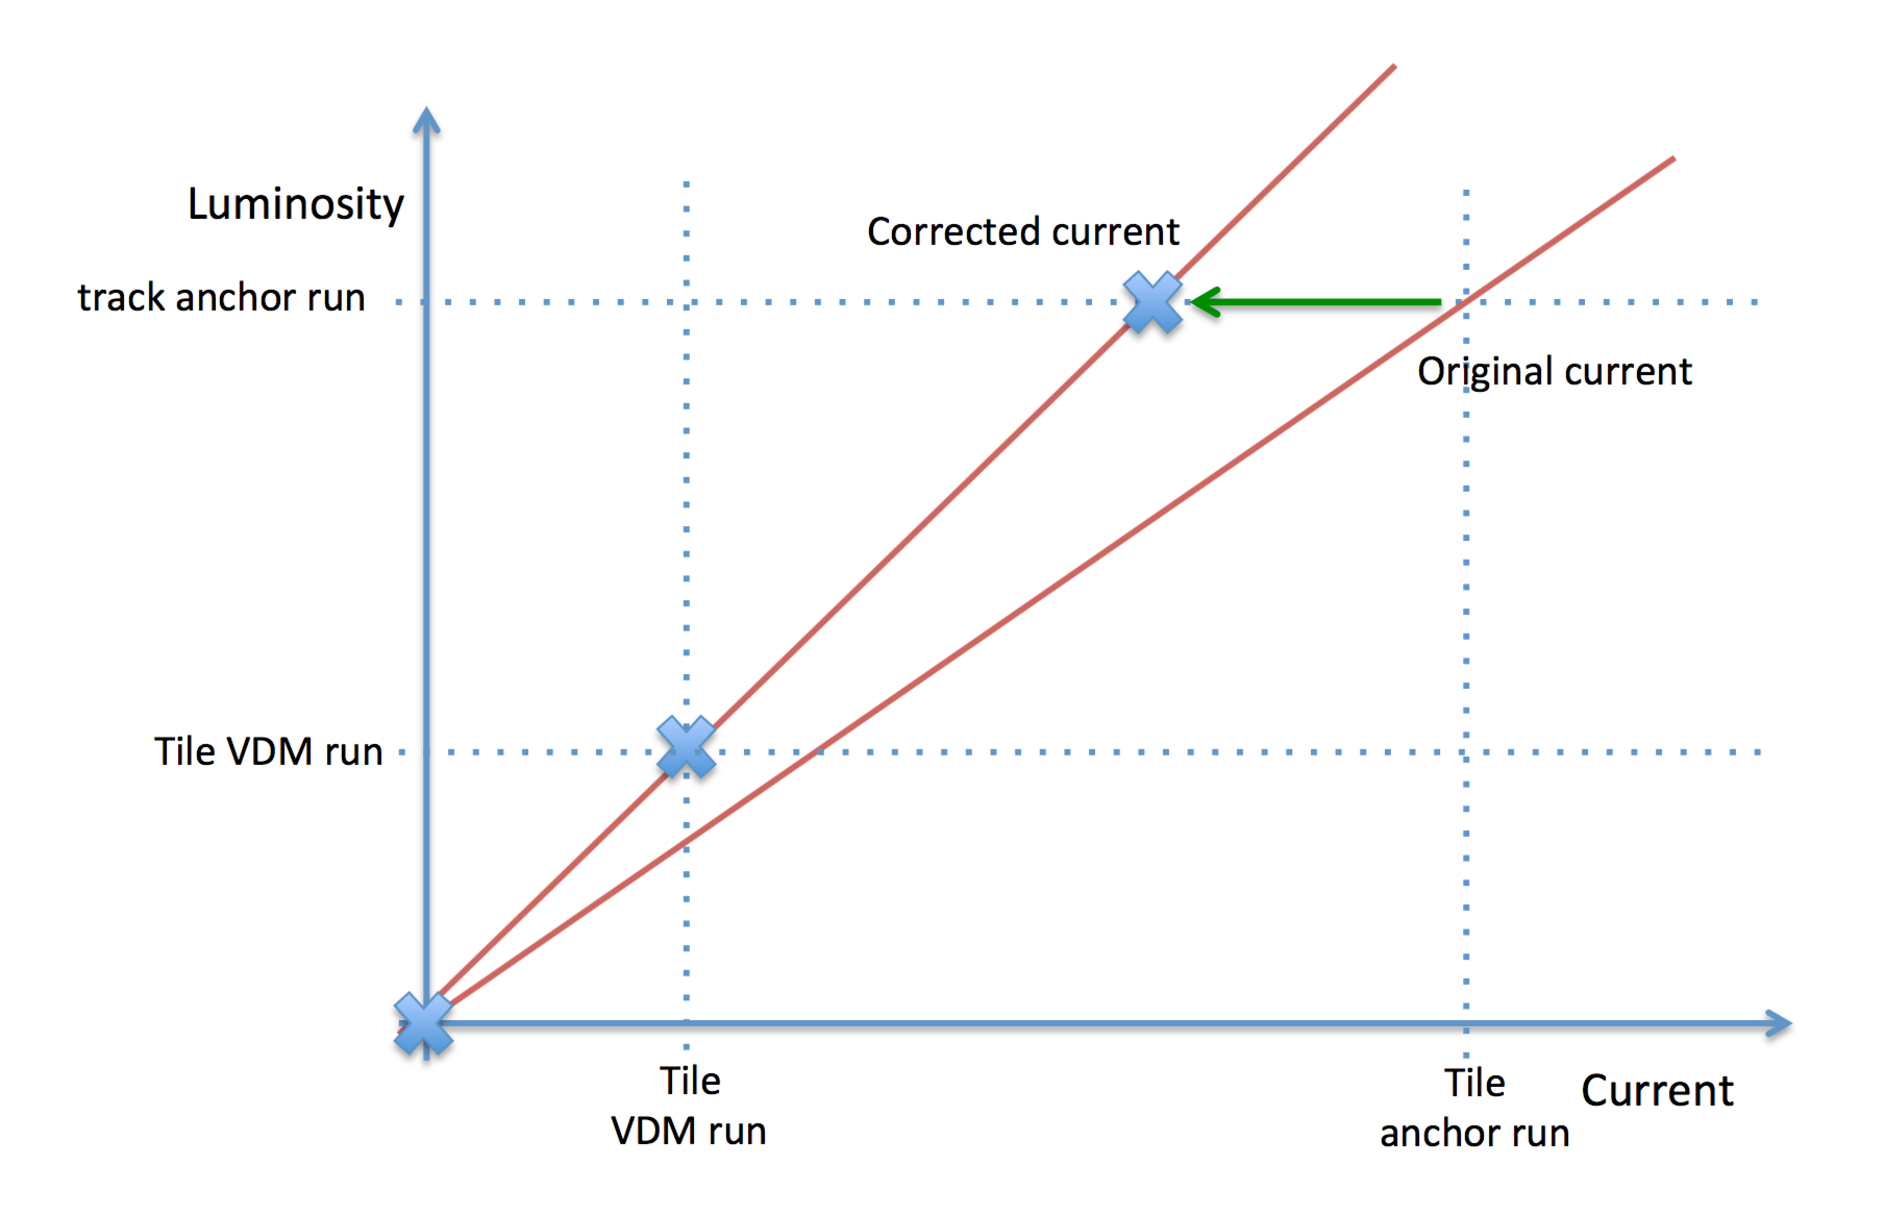
\includegraphics[width=0.65\textwidth]{figures/pmt_response/sketch.pdf}}
\caption{Schematic effect of the correction of the \gls{pmt} response on the \gls{tilecal} luminosity measurement.}
\label{fig:apppmt:sketch}
\end{figure}


\section{Conclusion}

The effect a non-linearity in the \gls{pmt} response with the increase in luminosity in the calibration transfer uncertainty from 
\gls{tilecal} has been studies. 
The calibration transfer uncertainty is the major source of uncertainty in the \gls{atlas} luminosity 
measurement, and it has a relevant impact for analyses that rely on a precise luminosity measurement. 
A correction has been derived, that allowed to reduce the calibration transfer uncertainty by XX \%.
This correction has been applied to the computation of the luminosity uncertainty released in March 2018, 
leading to a total luminosity uncertainty of 2.4\% on the 2017 data-taking periods. 


